\subsection{Apollo Server and Client}\label{subsection:background:graphql:apollo-server-client}

GraphQL has a specification and is a query language. Developing a GraphQL server and client is up to the application developer. Facebook has created its own GraphQL implementation of the specification in JavaScript with GraphQL.js for the backend and Relay for the frontend. Relay is a prominent example of a GraphQL client, but it is only available for Facebook's React framework. When evaluating different GraphQL clients, Apollo was chosen because it supports almost every possible programming language and framework.

\bigskip

\noindent Apollo Server is an open-source implementation of the GraphQL specification, and it offers any feature that the GraphQL specification states. Moreover, it supports \textbf{Apollo Sandbox} out of the box. \cite{misc:-:background:graphql:apollo-server-introduction} \textbf{Apollo Sandbox} helps local development. \textbf{Apollo Sandbox} loads the GraphQL Schema from the server with the help of the Introspection Query. \cite{misc:-:background:graphql:apollo-sandbox} Such a development environment enables executing queries and mutations directly inside the browser.

\bigskip

\noindent Apollo Client is a community-driven project with npm packages for almost all frontend development environments like Angular, React, and Vue.js. The library fetches, caches, and manages the data of the application. The package for Angular is designed with Angular patterns in mind to integrate perfectly with the framework. Apollo Client offers the possibility to cache already made requests. \cite{misc:-:background:graphql:apollo-angular-client-overview} \cite{misc:-:background:graphql:apollo-client-overview} Caching is especially important as it reduces the number of roundtrips to the server. The inner workings of the cache to prove or disprove the hypothesis are explained in the following sections.

\subsubsection{How does the in-memory cache work?}\label{subsubsection:background:graphql:apollo-server-client:in-memory-cache-working}

This section describes how the caching mechanism of the Apollo Client works. The structure of the cache is a local, normalized, in-memory cache. All GraphQL requests made with Apollo Client are cached inside the browser's memory by default. The cache enables Apollo Client to respond almost immediately to queries for already-cached data without sending a network request. This mechanism is needed to reduce round-trips to the server in subsequent requests of the same query because the requested data can be served from the cache. \cite{misc:-:background:graphql:apollo-client-cache-overview} Caching mechanisms generally reduce the server's load but introduce issues with cache management.

\bigskip

\noindent \textbf{Apollo Client} includes a caching interface called Apollo Cache and a proprietary implementation named \texttt{InMemoryCache}. Several Open-Source alternatives implement the ApolloCache interface, but Apollo's implementation is well-supported and receives regular updates.

\bigskip

\noindent Figure~\ref{fig:background:graphql:user-query-first-time} shows an exemplary query to fetch a user with its unique id. First, the Apollo Client checks whether the user with the given id is already stored inside the cache. If the query with that id has yet to be executed, a network query to fetch the user must be made. The result from the GraphQL Server is stored inside the cache and returned to the application. Four steps must be made to render data on the screen. \cite{misc:-:background:graphql:apollo-client-cache-overview}

\ifshowImages
\begin{figure}[H]
    \centering
    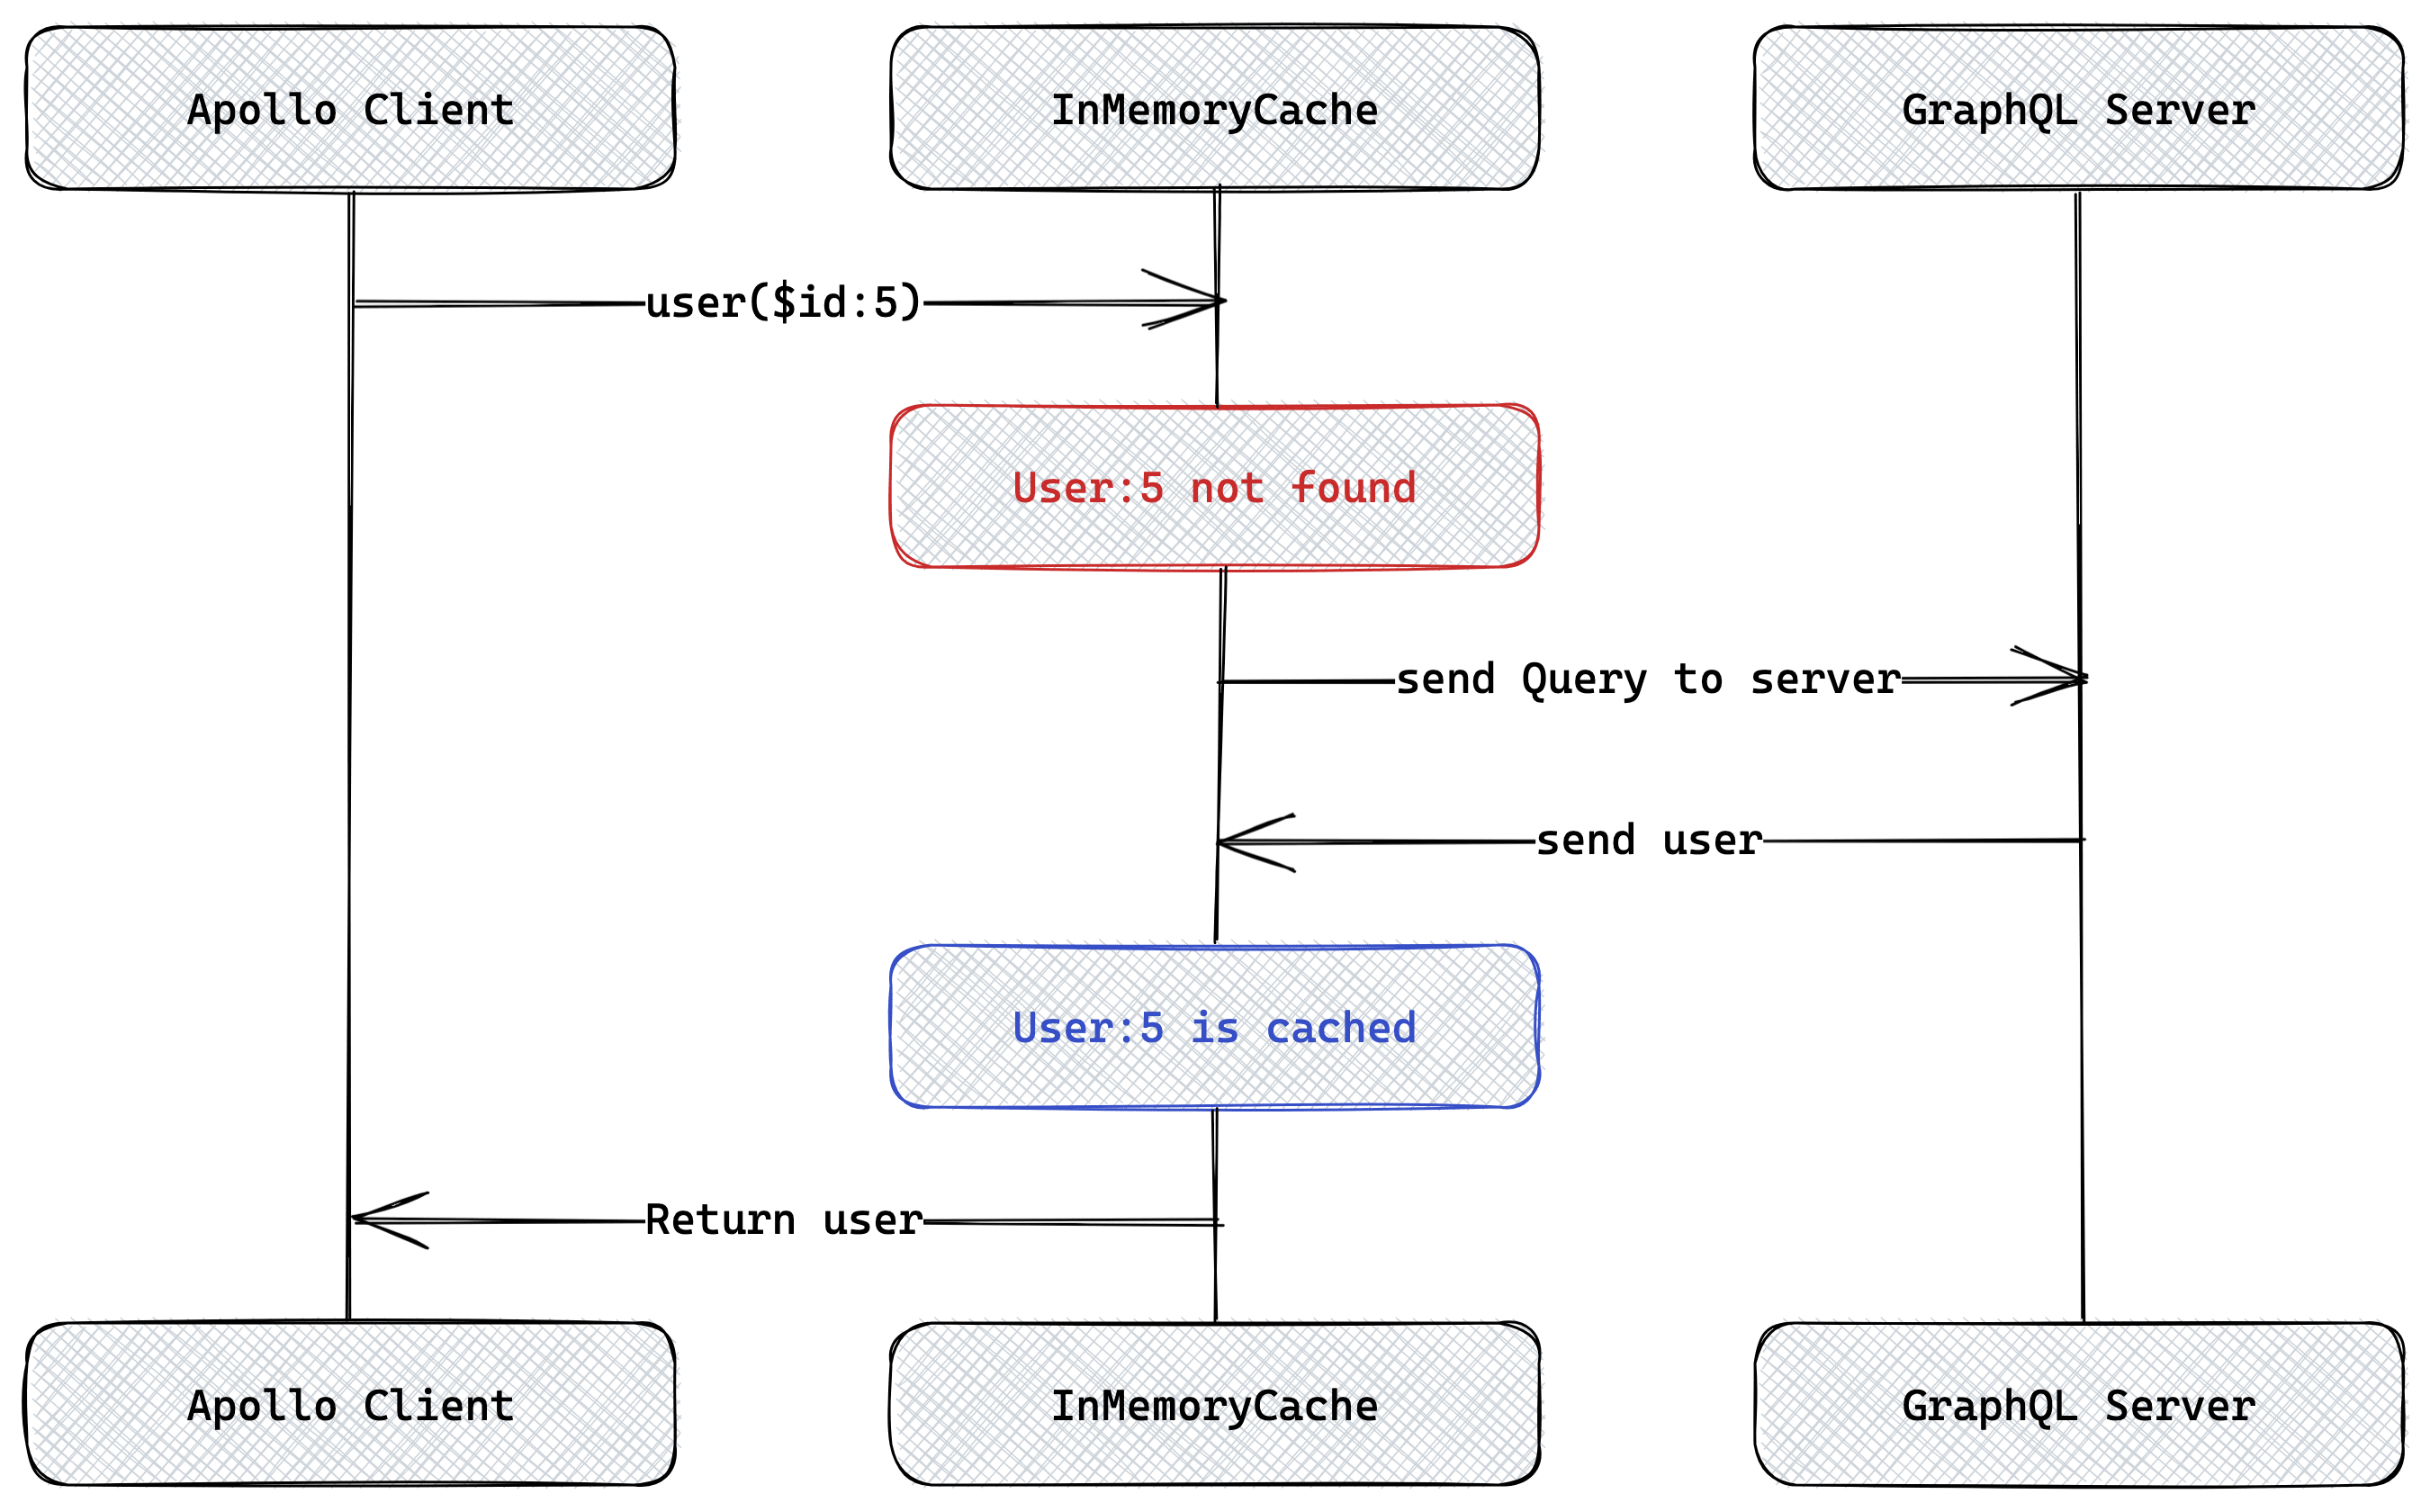
\includegraphics[width=0.6\linewidth]{images/background/apollo/apollo-client-basic-cache.png}
    \caption{The execution of a query which is not in the cache (Adapted from \cite{misc:-:background:graphql:apollo-client-cache-overview})}\label{fig:background:graphql:user-query-first-time}
\end{figure}
\fi

\noindent If a request with the same user id is made again, the flow of execution looks like in figure \ref{fig:background:graphql:user-query-second-time}. As seen in the figure, no network request has to be made to the GraphQL API, because everything is served from the Apollo Cache alone. Compared to the four steps in figure \ref{fig:background:graphql:user-query-first-time}, only two steps need to be done here. \cite{misc:-:background:graphql:apollo-client-cache-overview}

\ifshowImages
\begin{figure}[H]
    \centering
    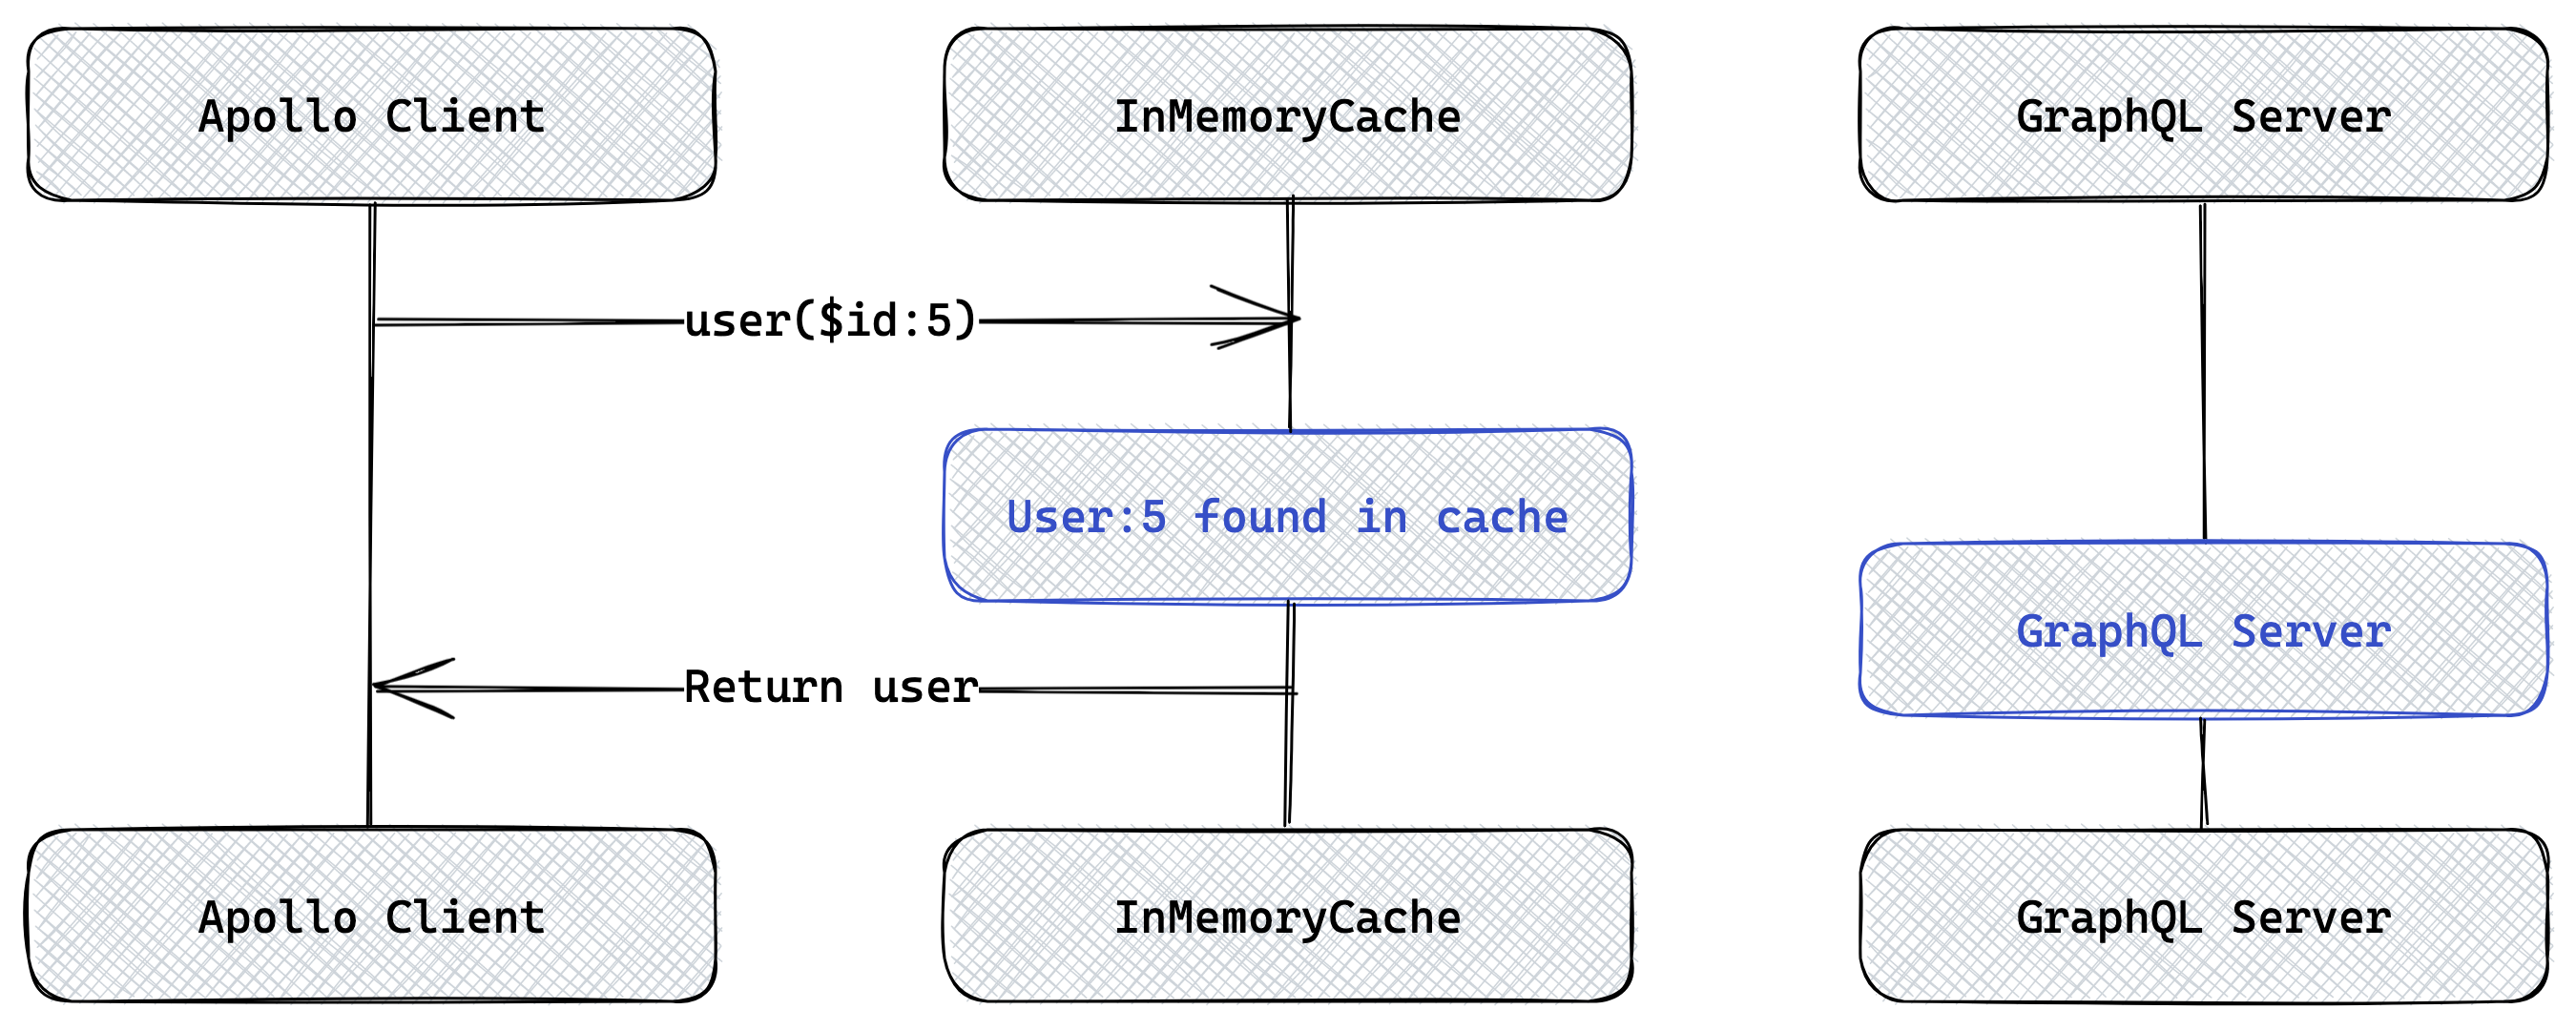
\includegraphics[width=0.7\linewidth]{images/background/apollo/apollo-client-basic-cache-warm.png}
    \caption{Executing the same query again reduces the steps. (Adapted from \cite{misc:-:background:graphql:apollo-client-cache-overview})}\label{fig:background:graphql:user-query-second-time}
\end{figure}
\fi

\subsubsection{Data normalization}\label{subsubsection:background:graphql:apollo-server-client:data-normalization}

Whenever the Apollo Client receives the response data of a query, it does the following. In order to correctly understand cache updates, it is essential to the structure of the cache before. The \texttt{InMemoryCache} is a simple normalized JavaScript object. The Apollo Client stores the data as a flat lookup table of objects referencing each other. An empty cache is just an empty object. These objects correspond to the objects that are returned by GraphQL queries. A single cache object might include fields fetched by multiple queries, allowing multiple queries to fetch different fields for the same object. \cite{misc:-:background:graphql:apollo-client-cache-overview} The following paragraphs describe the steps from a GraphQL query to the objects inside the cache.

\paragraph{1. Identify objects}\label{paragraph:background:graphql:apollo-server-client:data-normalization:identify-objects}

The cache identifies all distinct objects included in the query response. For example, take the query from figure \ref{code:background:graphql:query-user-cache}, which returns the \texttt{id}, \texttt{username}, and \texttt{email} of every user.

\ifshowListings
\begin{listing}[H]
    \begin{minted}{typescript}
query {
  users {
    id
    username
    email
  }
}
    \end{minted}
    \caption{A query that fetches the id, username, and email of every user.}\label{code:background:graphql:query-user-cache}
\end{listing}
\fi

The server responds with the following result from listing \ref{code:background:graphql:query-user-response-result}. The \texttt{\_\_typename} property is automatically appended to the query by the Apollo Client to identify the object.

\ifshowListings
\begin{listing}[H]
    \begin{minted}{typescript}
{
  users: [
    {
      __typename: 'User',
      id: '36bad921-8fcf-4f33-9f29-0d3cd70205c8',
      username: 'Florian',
      email: 'florian@test.io'
    },
    {
      __typename: 'User',
      id: 'a2096556-9a4e-4994-9de8-86c9e85ed6a1',
      username: 'Lisa',
      email: 'lisa@test.io'
    }
  ]
}
    \end{minted}
    \caption{The result of the GraphQL query from listing \ref{code:background:graphql:query-user-cache}}\label{code:background:graphql:query-user-response-result}
\end{listing}
\fi

The caching mechanism identifies the following objects to be cached.

\begin{itemize}
    \item A \texttt{User} with id \texttt{36bad921-8fcf-4f33-9f29-0d3cd70205c8}
    \item A \texttt{User} with id \texttt{a2096556-9a4e-4994-9de8-86c9e85ed6a1}
\end{itemize}

\paragraph{2. Generate cache IDs}\label{paragraph:background:graphql:apollo-server-client:data-normalization:generate-cache-ids}

After identifying all objects, the cache generates a cache ID for each object. A cache ID uniquely identifies a particular object while it is in the \texttt{InMemoryCache}.

\noindent So, the cache IDs for the objects from the previous section are:

\begin{itemize}
    \item \texttt{User:36bad921-8fcf-4f33-9f29-0d3cd70205c8}
    \item \texttt{User:a2096556-9a4e-4994-9de8-86c9e85ed6a1}
\end{itemize}

\noindent By default, an object's cache ID is concatenated with the object's \texttt{\_\_typename} and \texttt{id} (or \texttt{\_id}) fields. If the cache cannot generate a cache ID for a particular object, that object is directly stored inside its parent object and must be referenced via the parent. Therefore the cache is not always completely flat. This behavior is shown with the query in listing \ref{code:background:graphql:no-id-query-user-cache}. 

\ifshowListings
\begin{listing}[H]
    \begin{minted}{typescript}
query {
  allUsers {
    id
    username
    Title {
      name
    }
  }
}
    \end{minted}
    \caption{Don't fetch the id of the title for the user.}\label{code:background:graphql:no-id-query-user-cache}
\end{listing}
\fi

\noindent The query from the listing misses the id field inside the Title field. Therefore the cache stores the Title object directly inside the user object. The result inside the cache is shown in the listing
\ref{code:background:graphql:no-id-query-user-cache-representation}. 

\ifshowListings
\begin{listing}[H]
    \begin{minted}{typescript}
{
  'User:36bad921-8fcf-4f33-9f29-0d3cd70205c8': {
    __typeName: 'User',
    id: '36bad921-8fcf-4f33-9f29-0d3cd70205c8',
    username: 'Florian',
    Title: {
      name: 'BSc.',
    },
  },
  'User:a2096556-9a4e-4994-9de8-86c9e85ed6a1': {
    __typeName: 'User',
    id: 'a2096556-9a4e-4994-9de8-86c9e85ed6a1',
    username: 'Lisa',
    Title: {
      name: 'BSc.',
    },
  }
}
    \end{minted}
    \caption{The structure inside the cache with the query from listing \ref{code:background:graphql:no-id-query-user-cache}}\label{code:background:graphql:no-id-query-user-cache-representation}
\end{listing}
\fi

\noindent Omitting IDs from a query should be avoided. If data of an un-normalized object has to be updated, every occurrence of the item in the cache has to be updated manually. It should be avoided that the same thing is queried, sometimes with an id and sometimes without, because \texttt{ApolloClient} will throw an error when trying to update the cache after such a query.

\paragraph{3. Replace object fields with references}\label{paragraph:background:graphql:apollo-server-client:data-normalization:replace-object-fields-with-references}

Next, the cache takes each field that contains an object and replaces its value with a reference to the appropriate object. Listing \ref{code:background:graphql:nested-query-user-cache} shows a query that demonstrates how the objects from a query are transformed in the InMemoryCache representation.

\ifshowListings
\begin{listing}[H]
    \begin{minted}{typescript}
query {
  allUsers {
    id
    username
    Title {
      id
      name
    }
  }
}
    \end{minted}
    \caption{A query to demonstrate object replacement with references.}\label{code:background:graphql:nested-query-user-cache}
\end{listing}
\fi

Listing \ref{code:background:graphql:nested-query-response-user-cache} shows a single result from the GraphQL server for the query from listing \ref{code:background:graphql:nested-query-user-cache}.

\ifshowListings
\begin{listing}[H]
    \begin{minted}{typescript}
{
  __typename: 'User',
  id: '36bad921-8fcf-4f33-9f29-0d3cd70205c8',
  username: 'Florian',
  title: {
    __typename: 'Title',
    id: '2adb1120-d911-4196-ab1b-d5043cc7a00a',
    name: 'BSc.'
  }
},
    \end{minted}
    \caption{The result of the GraphQL query from listing \ref{code:background:graphql:nested-query-user-cache}.} \label{code:background:graphql:nested-query-response-user-cache}
\end{listing}
\fi

And listing \ref{code:background:graphql:nested-query-response-after-replacement} shows how the object is stored inside the InMemoryCache.

\ifshowListings
\begin{listing}[H]
    \begin{minted}{typescript}
{
  __typename: 'User',
  id: '36bad921-8fcf-4f33-9f29-0d3cd70205c8',
  username: 'Florian',
  title: {
    __ref: 'Title:36bad921-8fcf-4f33-9f29-0d3cd70205c8',
  }
},
    \end{minted}
    \caption{The result after the cache has replaced objects with references.}\label{code:background:graphql:nested-query-response-after-replacement}
\end{listing}
\fi

\noindent The \texttt{title} field now references the appropriate normalized \texttt{Title} object. If another \texttt{User} with the same \texttt{title} is stored inside the in-memory cache, that normalized \texttt{Title} object is reused. Normalization can drastically reduce data duplication inside the cache, and it also helps to make the data stay synchronous with the server.

\paragraph{4. Store normalized objects}\label{paragraph:background:graphql:apollo-server-client:data-normalization:store-normalized-objects}

The resulting objects are stored inside the cache's flat lookup table. Whenever an incoming object has the same cache ID as an existing cached object, the fields of those objects are merged. If the incoming and the existing object share existing fields, the incoming object overwrites the cached value for those fields. Fields that exist in only one object are preserved. This normalization constructs a partial copy of the graph on our client. \cite{misc:-:background:graphql:apollo-client-cache-overview}

\bigskip

\noindent Listing \ref{code:background:graphql:nested-query-user-cache-representation} shows how normalized objects are stored. Each user contains a reference to a title. Both users have the same title. Therefore the server returned duplicate data. However, the cache normalization causes the title to be only present once inside the cache. This behavior is constructive because when a cache item is updated, the entire cache object does not have to be traversed in search of the instance that has been changed. Only a single item has to be updated. The cache normalization works when the query contains either a \texttt{\_id} or \texttt{id} field.

\ifshowListings
\begin{listing}[H]
    \begin{minted}{typescript}
{
  'User:36bad921-8fcf-4f33-9f29-0d3cd70205c8': {
    __typeName: 'User',
    id: '36bad921-8fcf-4f33-9f29-0d3cd70205c8',
    username: 'Florian',
    Title: {
      __ref: 'Title:2adb1120-d911-4196-ab1b-d5043cc7a00a',
    },
  },
  'User:a2096556-9a4e-4994-9de8-86c9e85ed6a1': {
    __typeName: 'User',
    id: 'a2096556-9a4e-4994-9de8-86c9e85ed6a1',
    username: 'Lisa',
    Title: {
      __ref: 'Title:2adb1120-d911-4196-ab1b-d5043cc7a00a',
    },
  }
  'Title:2adb1120-d911-4196-ab1b-d5043cc7a00a': {
    __typeName: 'Title',
    id: '2adb1120-d911-4196-ab1b-d5043cc7a00a',
    name: 'BSc.',
  },
}
    \end{minted}
    \caption{The data inside the cache with the response from the query from listing \ref{code:background:graphql:nested-query-user-cache}.}\label{code:background:graphql:nested-query-user-cache-representation}
\end{listing}
\fi

\subsubsection{Understanding the structure of the cache}\label{subsubsection:background:graphql:apollo-server-client:understanding-cache-structure}

Apollo offers development tools for the browser in the form of browser extensions. The \textbf{Apollo Client Developer Tools} can be installed for Chrome and Firefox. The extension can be found in the Chrome Web Store and the Firefox Add-ons Store. The browser extension adds a tab to the browser inspection tools. \cite{misc:-:background:graphql:apollo-developer-tools} The view of the cache contents from the Apollo Client Development Tools can be seen in figure \ref{fig:background:graphql:apollo:apollo-dev-tools}.

\ifshowImages
\begin{figure}[H]
    \centering
    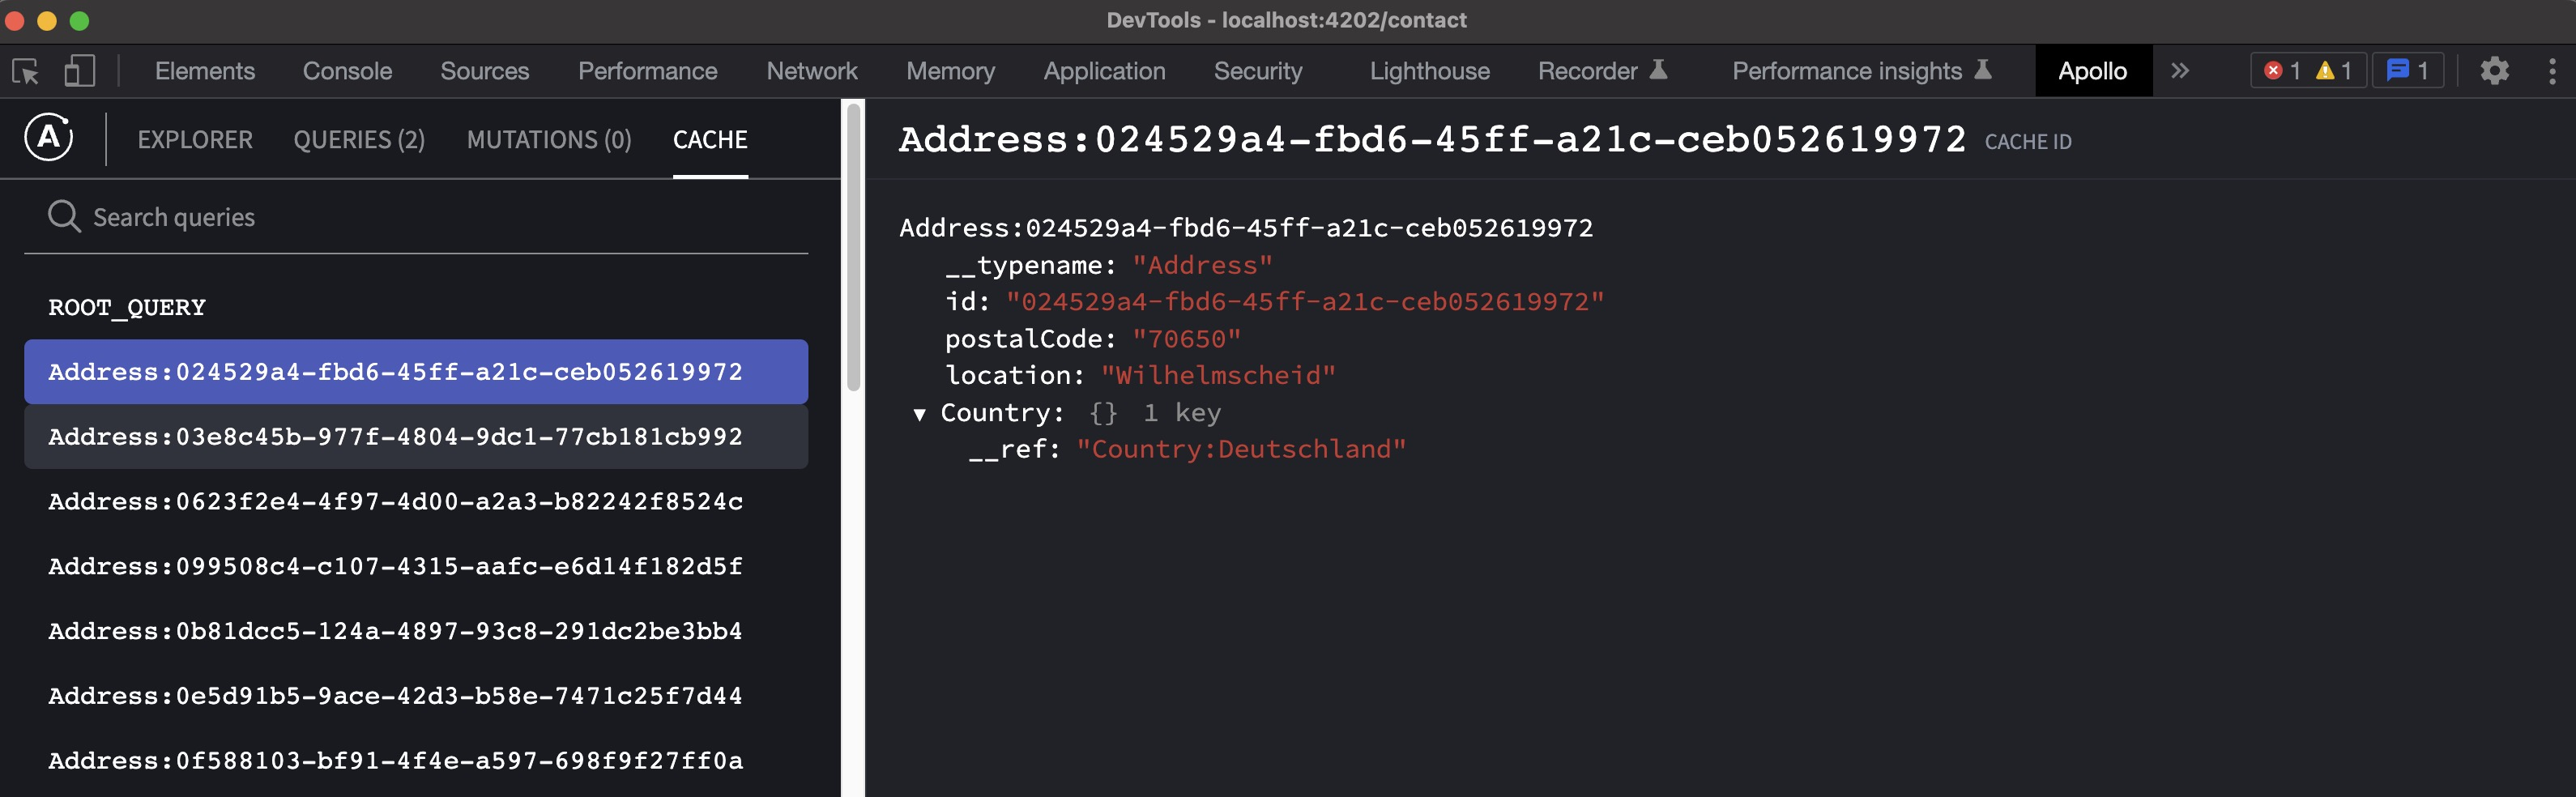
\includegraphics[width=1\linewidth]{images/background/apollo/apollo-dev-tools.jpeg}
    \caption{The content of the cache inside the Apollo Client Developer Tools}\label{fig:background:graphql:apollo:apollo-dev-tools}
\end{figure}
\fi

\noindent The development tools offer the following four main features: \cite{misc:-:background:graphql:apollo-developer-tools}

\begin{itemize}
    \item \textbf{GraphiQL}: Send queries to the server through the web application's configured Apollo Client instance, or query the Apollo Client cache to see what data is loaded.
    \item \textbf{Watched query inspector}: View active queries, variables, cached results, and re-run individual queries.
    \item \textbf{Mutation inspector}: View active mutations and their variables, and re-run individual mutations.
    \item \textbf{Cache inspector}: Visualize the Apollo Client and search it by field name and/or value.
\end{itemize}

\noindent Another method to access the content of the cache is through the \texttt{window} object in JavaScript. The object can be accessed through \texttt{window.\_\_APOLLO\_CLIENT\_\_.cache.extract()} inside the browser's development console.

\ifshowImages
\begin{figure}[H]
    \centering
    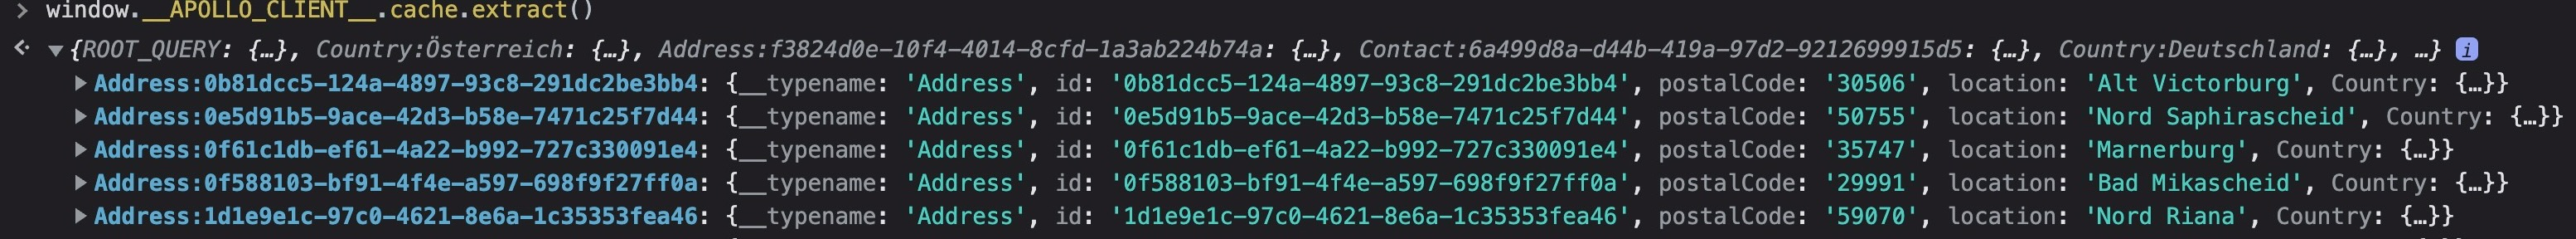
\includegraphics[width=1\linewidth]{images/background/apollo/apollo-cache-browser-window.jpeg}
    \caption{Viewing the contents of the cache inside the development console}\label{fig:background:graphql:apollo:apollo-cache-browser-window}
\end{figure}
\fi

\noindent  With this approach, the content of the cache can be explored with the help of JavaScript methods inside the browser development tools.

% ---

% The \textbf{Apollo Client} will update the cache so that it looks like this.

% \ifshowListings
% \begin{listing}[H]
%     \begin{minted}{typescript}
% {
%   ROOT_QUERY: {
%     __typename: 'Query',
%     users: [
%       { __ref: 'User:36bad921-8fcf-4f33-9f29-0d3cd70205c8', },
%       { __ref: 'User:a2096556-9a4e-4994-9de8-86c9e85ed6a1', },
%     ],
%   },
%   'User:36bad921-8fcf-4f33-9f29-0d3cd70205c8': {
%     __typeName: 'User',
%     id: '36bad921-8fcf-4f33-9f29-0d3cd70205c8',
%     username: 'Florian',
%     email: 'florian@test.io',
%   },
%   'User:a2096556-9a4e-4994-9de8-86c9e85ed6a1': {
%     __typeName: 'User',
%     id: 'a2096556-9a4e-4994-9de8-86c9e85ed6a1',
%     username: 'List',
%     email: 'list@test.io',
%   }
% }
%     \end{minted}
%     \caption{The data inside the cache with the response from listing \ref{code:background:graphql:query-user-response-result}}\label{code:background:graphql:query-user-cache-representation}
% \end{listing}
% \fi

% Let's describe how the response from the server is transformed into the representation from the cache seen in listing \ref{code:background:graphql:query-user-cache-representation}. The cache object contains a key \textbf{ROOT\_QUERY}. This element contains the name of the queries that were executed and the results from all queries. The query \textbf{allUsers} was fetched, therefore the \textbf{ROOT\_QUERY} contains a field with the name \textbf{users}. The listing \ref{code:background:graphql:query-user-cache-representation} shows that the content of the \textbf{ApolloClient} is clearly different from the servers response. Instead of the user-information every array item consists of an object with a \textbf{\_\_ref} key. The value of the key is simply the \textbf{\_\_typename} and \textbf{id} of the user concatenated. The data from the response has been normalized and added to the cache object. Next to the \textbf{ROOT\_QUERY} element, the actual user-information is stored. Each has the same key as the \textbf{\_\_ref} from the \textbf{ROOT\_QUERY}.

% \bigskip

% \noindent The same principle applies to arbitrary deep queries. The following query produces:

% \noindent And the server responds with the following result. The \textbf{\_\_typename} property is automatically appended to the query by the \textbf{ApolloClient}.

% \ifshowListings
% \begin{listing}[H]
%     \begin{minted}{typescript}
% {
%   users: [
%     {
%       __typename: 'User',
%       id: '36bad921-8fcf-4f33-9f29-0d3cd70205c8',
%       username: 'Florian',
%       title: {
%         __typename: 'Title',
%         id: '2adb1120-d911-4196-ab1b-d5043cc7a00a',
%         name: 'BSc.'
%       }
%     },
%     {
%       __typename: 'User',
%       id: 'a2096556-9a4e-4994-9de8-86c9e85ed6a1',
%       username: 'Lisa',
%       title: {
%         __typename: 'Title',
%         id: '2adb1120-d911-4196-ab1b-d5043cc7a00a',
%         name: 'BSc.'
%       }
%     }
%   ]
% }
%     \end{minted}
%     \caption{The result of the GraphQL query from listing \ref{code:background:graphql:nested-query-user-cache}}\label{code:background:graphql:nested-query-user-response-result}
% \end{listing}
% \fi

% The \textbf{ROOT\_QUERY} is exactly the same as with the query before.  Without an id the object can't be normalized. Here is an example:

% The response:

% \ifshowListings
% \begin{listing}[H]
%     \begin{minted}{typescript}
% {
%   users: [
%     {
%       __typename: 'User',
%       id: '36bad921-8fcf-4f33-9f29-0d3cd70205c8',
%       username: 'Florian',
%       title: {
%         __typename: 'Title',
%         name: 'BSc.'
%       }
%     },
%     {
%       __typename: 'User',
%       id: 'a2096556-9a4e-4994-9de8-86c9e85ed6a1',
%       username: 'List',
%       title: {
%         __typename: 'Title',
%         name: 'BSc.'
%       }
%     }
%   ]
% }
%     \end{minted}
%     \caption{The result of the GraphQL query from listing \ref{code:background:graphql:no-id-query-user-cache}}\label{code:background:graphql:no-id-query-user-response-result}
% \end{listing}
% \fi
